\documentclass[11pt,a4paper]{article}

% --- Packages ---
\usepackage[english]{babel}
\usepackage{geometry}
\geometry{margin=2.5cm} % Standard professional margins
\usepackage{graphicx} % For inserting figures
\usepackage{booktabs} % For beautiful tables
\usepackage{listings} % For code snippets
\usepackage{xcolor}   % For code highlighting colors
\usepackage{fontspec} % Required to use custom system fonts like Consolas
\usepackage{hyperref} % For clickable links and references
\usepackage{lipsum}   % Can be removed (used here for placeholder text)
\usepackage{array}
\usepackage{subcaption}
\usepackage{float}
\usepackage{tikz}
\usepackage{xcolor}
\usetikzlibrary{shapes.geometric, arrows.meta, positioning, fit, backgrounds}

\hyphenpenalty=10000
\exhyphenpenalty=10000
\sloppy

% --- Visual Studio Dark Theme Colors ---
\definecolor{vsBackground}{HTML}{1E1E1E}  % Dark background
\definecolor{vsText}{HTML}{D4D4D4}        % Light gray default text
\definecolor{vsKeyword}{HTML}{569CD6}     % Blue for keywords (public, class, private)
\definecolor{vsType}{HTML}{4EC9B0}        % Teal for Types/Classes (LLMRepository)
\definecolor{vsInterface}{HTML}{B8D7A3}   % Light green for Interfaces (ILLMRepository)
\definecolor{vsString}{HTML}{D69D85}      % Terracotta/Brown for strings ("LLMApiKey")
\definecolor{vsComment}{HTML}{57A64A}     % Green for comments
\definecolor{vsNumber}{HTML}{B5CEA8}      % Light green for numbers (1000, 60)
\definecolor{vsLineNum}{HTML}{2B91AF}     % Muted teal for line numbers

% --- Setup the Code Font ---
% Consolas is a proprietary Microsoft font. If compiling on Overleaf, 
% you can use 'Courier New' or upload a Consolas .ttf file, or use 'Fira Code'.
\newfontfamily\vsCodeFont[
    Path=fonts/,
    Extension=.TTF,
    Scale=0.9
]{CASCADIAMONO} % Loading Consolas from fonts directory

% --- Define C# Language with Common Keywords ---
\lstdefinelanguage{CSharp}[Sharp]{C}{
    morekeywords={
        abstract, as, base, break, case, catch, checked, class, const, continue,
        default, delegate, do, else, enum, event, explicit, extern, false, finally,
        fixed, for, foreach, goto, if, implicit, in, interface, internal, is, lock,
        namespace, new, null, object, operator, out, override, params, private,
        protected, public, readonly, ref, return, sealed, sizeof, stackalloc, static,
        string, struct, switch, this, throw, true, try, typeof, unchecked, unsafe,
        using, virtual, void, volatile, while, async, await, var, dynamic, yield,
        get, set, value, where, select, from, let, orderby, group, join, into
    },
    % Common .NET types - automatically colored as types
    morekeywords=[2]{
        String, Int32, Int64, Boolean, Double, Float, Decimal, Byte, Char, Object,
        Task, List, Dictionary, IEnumerable, ICollection, IList, IDictionary,
        HttpClient, HttpResponseMessage, HttpRequestException, StringBuilder,
        DateTime, TimeSpan, Guid, Exception, ArgumentException, InvalidOperationException
    },
    % Add your custom interfaces here - they'll be colored differently
    morekeywords=[3]{
        ILLMRepository, IRepository, IService, IDisposable
    },
    % Add your custom classes here
    morekeywords=[4]{
        LLMRepository, Policy
    },
    sensitive=true,
    morecomment=[l]{//},
    morecomment=[s]{/*}{*/},
    morecomment=[s][keywordstyle]{[}{]}, % Attributes
    morestring=[b]",
}

% --- Apply Visual Studio Theme Settings ---
\lstset{
    language=CSharp,
    backgroundcolor=\color{vsBackground},   
    basicstyle=\vsCodeFont\small\color{vsText},
    commentstyle=\color{vsComment}\itshape,
    keywordstyle=\color{vsKeyword},          % Blue for keywords
    keywordstyle=[2]\color{vsType},          % Teal for .NET types
    keywordstyle=[3]\color{vsInterface},     % Light green for interfaces
    keywordstyle=[4]\color{vsType},          % Teal for custom classes
    stringstyle=\color{vsString},
    numberstyle=\tiny\color{vsLineNum},
    % Structural layout
    breakatwhitespace=false,         
    breaklines=true,                 
    captionpos=b,                    
    keepspaces=true,                 
    numbers=left,                    
    numbersep=8pt,                  
    showspaces=false,                
    showstringspaces=false,
    showtabs=false,                  
    tabsize=4,
    frame=single,
    rulecolor=\color{vsBackground}
}

% --- Hyperref Setup ---
\hypersetup{
    colorlinks=true,
    linkcolor=black,
    filecolor=magenta,      
    urlcolor=cyan,
    citecolor=cyan,
}


% ==========================================
% INFO
% ==========================================
\title{Internship Report PercursusAPI BE + FE}
\author{Hugo Simas de Melo}
\date{June 2026}

\begin{document}


% ==========================================
% CAPA
% ==========================================
\begin{titlepage}
    \centering

    {
\includegraphics[width=0.5\textwidth]{images/logo_up.png}}
    {
\includegraphics[width=0.35\textwidth]{images/logo_craftable.png}}
    
    \vspace*{5cm}
    
    {\LARGE\bfseries PercursusAPI BE + FE}\\[0.8cm]
    {\Large\bfseries\itshape Internship report}\\[2.5cm]
    
    {\large\textbf{Author:}}\\[0.1cm]
    {\large Hugo Simas de Melo\\[0.1cm]
    (Student ID: 202304068)}\\[1.5cm]
    
    {\large\textbf{Supervisor:}}\\[0.1cm]
    {\large Artur Peniche}
    
    \vfill
    
    {\small Faculdade de Ciências da Universidade do Porto}\\
    {\small craftable software}\\[0.5cm]
    {\large Porto, June 29, 2026}
\end{titlepage}

\newpage


% ==========================================
% TABLE OF CONTENTS
% ==========================================
\tableofcontents
\newpage


% ==========================================
% 1. INTRODUCTION
% ==========================================
\section{Introduction}
\label{sec:introduction}


% ==========================================
% 1.1 Context and Objectives
% ==========================================
\subsection{Context and Objectives}
\label{sub:context}

This internship focused on developing and improving the features of the Percursus mobile application.
Its goal is to offer new forms of interaction between users and their surroundings through trails, along which users can complete trivia-style activities about different Points of Interest (POI) in exchange for points.
The application is still in the development stage but has emerged in response to the growing popularity of activities such as geocaching and increasing investment by municipalities in developing and maintaining trails.


% ==========================================
% 1.2 Host Institution
% ==========================================
\subsection{Host Institution}
\label{sub:company_profile}

The internship was conducted at craftable software, a boutique custom software development house founded in 2020.
Headquartered and operating mostly on a remote-hybrid model in Porto and Aveiro, the company specializes in engineering high-quality, reliable, and scalable digital solutions for an international client base in Europe and the United States.

The company employs a multidisciplinary team of senior engineers, product designers, and delivery leaders.
The organization provides consulting and outsourced technical services in diverse sectors, including healthcare, fintech, retail, and travel technology. ~\cite{craftable2026}

Engineering teams focus on cloud-native systems, DevSecOps pipelines, agile methodologies, and robust automation testing.
The company's core technological expertise aligns precisely with the full-stack paradigm used during this internship, focusing specifically on enterprise backend engineering with C\# (.NET Core) and dynamic frontend interfaces using React.

\vspace*{0.5cm}

% ==========================================
% 2. State of The Art
% ==========================================
\section{State of the Art}
\label{sec:sota}
 
Percursus sits at the intersection of three active and evolving product domains: location-based mobile applications, gamification mechanics and social features in mobile applications.


% ==========================================
% 2.1 Location Based Mobile Apps
% ==========================================
\subsection{Location-Based Mobile Applications}
\label{sub:sota:location}
 
Location-based mobile applications have evolved significantly beyond simple map navigation.
The genre was popularized at scale by Pokémon GO, which normalized the expectation that the physical world should \textit{respond} to the user's presence through a persistent progression system and live map-driven interaction~\cite{edgeorbital2026geocaching}.
In 2026, the category spans a spectrum from traditional cache-hunting platforms, such as Geocaching and c:geo, to gamified exploration apps and real-world mission systems.
The dominant trend across the category is a shift from apps that \textit{log where you went} to platforms that make the physical world feel active and reactive~\cite{edgeorbital2026geocaching}.
 
The hiking and trail app genre is one of the fastest-growing niches in the outdoor mobile app market.
The global hiking app market was valued at \$387.6 million in 2026 and is forecast to reach \$1.02 billion by 2035, growing at a Compound Annual Growth Rate (CAGR) of 11.4\,\%~\cite{markwide2026hiking}.
Leading platforms such as AllTrails, which aggregates over 500,000 trails worldwide and serves both casual and technical hikers, illustrate the appetite for rich, location-anchored content delivered through a polished cross-platform mobile experience~\cite{alltrails2026}.
A key technical requirement emerging across this segment is \textit{offline-first} architecture: wilderness and trail environments frequently lack mobile connectivity, and market research identifies offline-first design as a baseline expectation for outdoor navigation products~\cite{markwide2026hiking}.
 

% ==========================================
% 2.2 Gamification
% ==========================================
\subsection{Gamification Mechanics in Mobile Applications}
\label{sub:sota:gamification}
 
Gamification, the integration of game-like mechanics such as points, badges, leaderboards, achievements, and progression systems into non-game contexts, has transitioned from a differentiating feature to a retention baseline in the mobile app market.
The global gamification market was valued at \$36.46 billion in 2026 and is projected to reach \$112.32 billion by 2031, at a CAGR of 25.24\,\%~\cite{startus2026gamification}.
Over 70\,\% of Global 2000 companies now deploy some form of gamification across their digital products~\cite{visu2026gamification}.
 
The evidence of its effectiveness in driving engagement is substantial.
Industry reports for 2025--2026 indicate that well-executed gamification results in a 54\,\% increase in daily active users (DAU), and gamified loyalty programs lift retention by 47\,\%~\cite{strivecloud2026gamification}.
Academic research published in the \textit{Journal of Marketing Research} confirms that game-based rewards increase user engagement significantly over value-based rewards alone, although the same research cautions that excessive gamification flow can distract users from the core value-added activities that the app is designed to support~\cite{ama2025gamification}.
 
The most effective modern implementations move beyond simple point accumulation toward \textit{hybrid reward architectures}: systems that combine intrinsic game progression (level-ups, streaks, achievement badges) with extrinsic context-aware rewards.
AI-enabled gamification, where the reward system adapts personalization to individual behaviour patterns, has been shown to achieve a 47\,\% increase in user interaction frequency and a 38\,\% improvement in retention compared to static systems ~\cite{amplifai2026gamification}.
Duolingo remains the canonical reference for retention-optimized gamification: by combining streaks, leaderboards, and AI-adapted feedback loops, it reduced user churn from 47\,\% to 28\,\% in major markets and sustained a 36\,\% year-on-year growth in DAUs~\cite{strivecloud2026duolingo}.
 
In location-based and outdoor exploration contexts, gamification serves an additional purpose beyond retention: it provides structured motivation for physical exploration.
Point systems and achievement tiers incentivize users to visit more locations and complete more activities, turning passive trail use into an active, goal-directed experience.


% ==========================================
% 2.3 Friends in Mobile Apps
% ==========================================
\subsection{Social and Friend Features in Mobile Applications}
\label{sub:sota:social}

Social features have become one of the most reliable drivers of retention in mobile applications, particularly in outdoor activity and fitness segments.
The evidence is consistent and significant: apps that successfully integrate social mechanics retain users at substantially higher rates than those that do not.
Fitness apps with social features achieve day-one retention rates of 30--35\,\% compared to 27\,\% for general health apps, and the gap widens considerably at the 30-day mark~\cite{lucid2025retention}.
Strava, the most studied example in this space, averages over 35 monthly sessions per user, more than double the figure of its outdoor competitors, a result attributed directly to its social architecture~\cite{sensortower2026strava}.
 
The most effective social designs for location-based and outdoor applications are built around three distinct mechanisms.
 
The first is \textbf{ contextualized competition}.
Rather than ranking all users on a single global leaderboard, which is demotivating for the majority who will never appear near the top, leading platforms decompose competition into smaller and locally meaningful contexts. 
Strava's segment system is the canonical example: every named stretch of trail becomes its own competitive arena, so an average athlete can hold the fastest time in their neighbourhood even if they rank nowhere globally~\cite{trophy2026strava}.
This design principle, which makes competitive achievability relative to the user's actual context rather than absolute ability, is directly applicable to trail-based applications with friend leaderboards, where showing a user their rank among friends is more motivating than showing them their rank among all platform users.
 
The second is \textbf{community and group formation}.
Strava's Year in Sport report recorded a 5.8x increase in hiking clubs in 2025, and the platform released a dedicated set of hiking-specific social features in June 2026, covering discovery, navigation, and social sharing~\cite{strava2026hiking}.
This confirms that hiking and trail activity is becoming an increasingly social behaviour and that platforms that facilitate group formation around shared routes and locations are capturing a growing segment of outdoor users.
Apps that only track individual performance without enabling friends to connect around the same trails leave a significant retention lever unused~\cite{feed2026fitness}.
 
The third is \textbf{friend-relative progress visibility}.
Industry data show that users who interact with social features complete more activities and maintain longer engagement streaks~\cite{lucid2025retention}.
Apps with social streak features, where progress is visible to connected users, show average streak lengths 34\,\% longer than apps without
them~\cite{trophy2026strava}.
The practical design implication is that showing users how they compare to specific friends (rather than anonymous strangers) creates a personally meaningful competitive context that generic leaderboards cannot replicate.
 
The state of the art for friend systems in mobile applications in 2026 therefore encompasses a friend request and connection flow, a friends-filtered leaderboard view, activity or progress visibility between connected users, and optionally social reactions or commentary on activity completions.
Platforms that implement only a basic friend list without surfacing friend data in contextually relevant moments do not capture the retention benefits that motivate the investment in social infrastructure in the first place~\cite{getstream2026social}.
 
\vspace*{0.5cm}

 
% ==========================================
% 3. Description of Work
% ==========================================
\section{Description of Work}
\label{sec:description}


% ==========================================
% 3.1 Workflow
% ==========================================
\subsection{Workflow}
\label{sub:workflow}

The \textbf{Atlassian} suite was consistently used as the enterprise-level development platform throughout the internship: \textbf{Jira} for issuing and managing tickets, \textbf{Confluence} for sharing and maintaining documentation artifacts, and \textbf{Bitbucket}, which is a Git-based code-hosting platform with built-in CI/CD pipelines.\\
 
Larger tasks were divided into multiple tickets following an \textbf{Agile} workflow.
Work was organized into two-week \textit{sprints}, at the end of which new tickets were assigned and the workload was reassessed to maintain a sustainable pace.
For two sprints, I transitioned to a \textbf{Kanban} approach, tackling tickets with more flexibility as they were created.
This is a common shift when a product moves from active development into production, where an increased flow of bug fixes and optimizations requires a more reactive process rather than fixed-sprint commitments.\\
 
The development cycle for each ticket followed a consistent branch-based flow: a feature branch was created from the base branch, changes were implemented and pushed, tests were created or updated to support the new implementation, the CI/CD pipeline automatically ran those same tests, and a pull request was opened for code review.
The supervisor reviewed the changes, suggested corrections or improvements, and approved the merge once the code met the required standard.\\

Although the application was split into four repositories: backend, frontend, Infrastructure as Code (IAC), and later a Content Management System (CMS), I only came into contact with the first two.
Two different Integrated Development Environments (IDEs) were used in parallel: \textbf{Microsoft Visual Studio} for the backend and \textbf{Visual Studio Code} for the frontend.
This choice was driven by tooling support: Visual Studio provides deeper integration for \textbf{C\#} development, while Visual Studio Code is better suited to \textbf{React Native} ecosystem.

\newpage

% ==========================================
% 3.2 Technical Foundation
% ==========================================
\subsection{Technical Foundation}
\label{sub:tech}

The first two weeks of the internship were spent learning the tools used for the project.
This included taking modules for technologies that I was unfamiliar with, such as the C\# programming tool through the Microsoft Learning Paths ~\cite{microsoftLearn} and the MongoDB database type through the MongoDB C\# Developer Path~\cite{mongoDBcSharp} that provided me with the basic foundations on how they worked and how to use them.


% ==========================================
% 3.2.1 Backend Architecture
% ==========================================
\subsubsection{Backend Architecture}
\label{subsub:tech:backend}

The backend is a \textbf{.NET} REST API structured around a layered N-Tier architecture using a Repository Design Pattern, which is divided into four main modules, each handling a single responsibility:

\begin{itemize}
    \item \textbf{\texttt{API} (Presentation):} Entry point of the application. Hosts HTTP controllers, custom middleware pipelines, and application configurations.

    \item \textbf{\texttt{Services} (Business Logic):} Contains the core application rules, data processing logic, and input validation. This layer is the only one with which the \texttt{API} layer communicates directly.

    \item \textbf{\texttt{Repositories} (Data Access):} Solely responsible for database interaction, keeping query logic isolated from business rules.

    \item \textbf{\texttt{Models}}: This layer held all of the DTOs (Data Transfer Objects) that traveled through the previously mentioned layers
\end{itemize}

The \textbf{Repository Pattern} hides data-access details behind interfaces, decoupling the service layer from database mechanics.
\textbf{Dependency Injection} with Singleton, Scoped, and Transient lifecycles keeps components loosely coupled and memory-managed by the framework.
Where multiple behaviours must be triggered dynamically (for example, dispatching a notification for an \texttt{Achievement} versus a \texttt{Walk} event), a \textbf{Factory} combined with \textbf{Strategy/Handler} objects replaces cumbersome switch-case logic with an extensible dispatch system.
Data flowing over the network is always shaped by \textbf{DTOs with custom mappers}, ensuring that internal database structures are never directly exposed to the client.
All layers use the \textbf{async/await} pattern (\texttt{Task<T>}), preventing thread-blocking on I/O-bound operations and maximizing API throughput.





\newpage

% ==========================================
% 3.2.3 Frontend Architecture
% ==========================================
\subsubsection{Frontend Architecture}
\label{subsub:tech:frontend}

The client is a cross-platform mobile application built with \textbf{React Native} on the \textbf{Expo} ecosystem and is written mostly in \textbf{TypeScript}.
The codebase follows a feature-based folder structure, and screen components never fetch data directly: all network calls are delegated to isolated service functions built on \textbf{Axios} that return strictly typed response models, mirroring the separation of concerns of the backend.

The global state is managed through React's native \textbf{Context API}, which is split into four domain-specific contexts: \texttt{UserContext} for authentication and profile sessions, \texttt{LocationContext} for real-time GPS streaming, \texttt{ConnectionContext} for network status monitoring, and \texttt{NotificationContext} for push notification token management.
This avoids the overhead of a monolithic global state library while keeping the shared state well-organized and explicit.

The application was designed with an \textbf{offline-first} approach in mind, combining background location tracking with local caching to preserve functionality when connectivity is lost.
However, successive upstream updates to React Native and the abandonment of a package used for caching broke the implementation in the early stage of the internship period, and the feature was moved to the backlog and effectively held in a stand-by [~\ref{subsub:updates}]

\subsection{Application Flow}
\label{sub:appflow}

% ==========================================
% Architecture Diagram - TikZ
% Add to preamble:
%   \usepackage{tikz}
%   \usepackage{xcolor}
%   \usetikzlibrary{arrows.meta, positioning, fit, backgrounds}
% ==========================================

\begin{figure}[ht]
\centering
\makebox[\textwidth][c]{
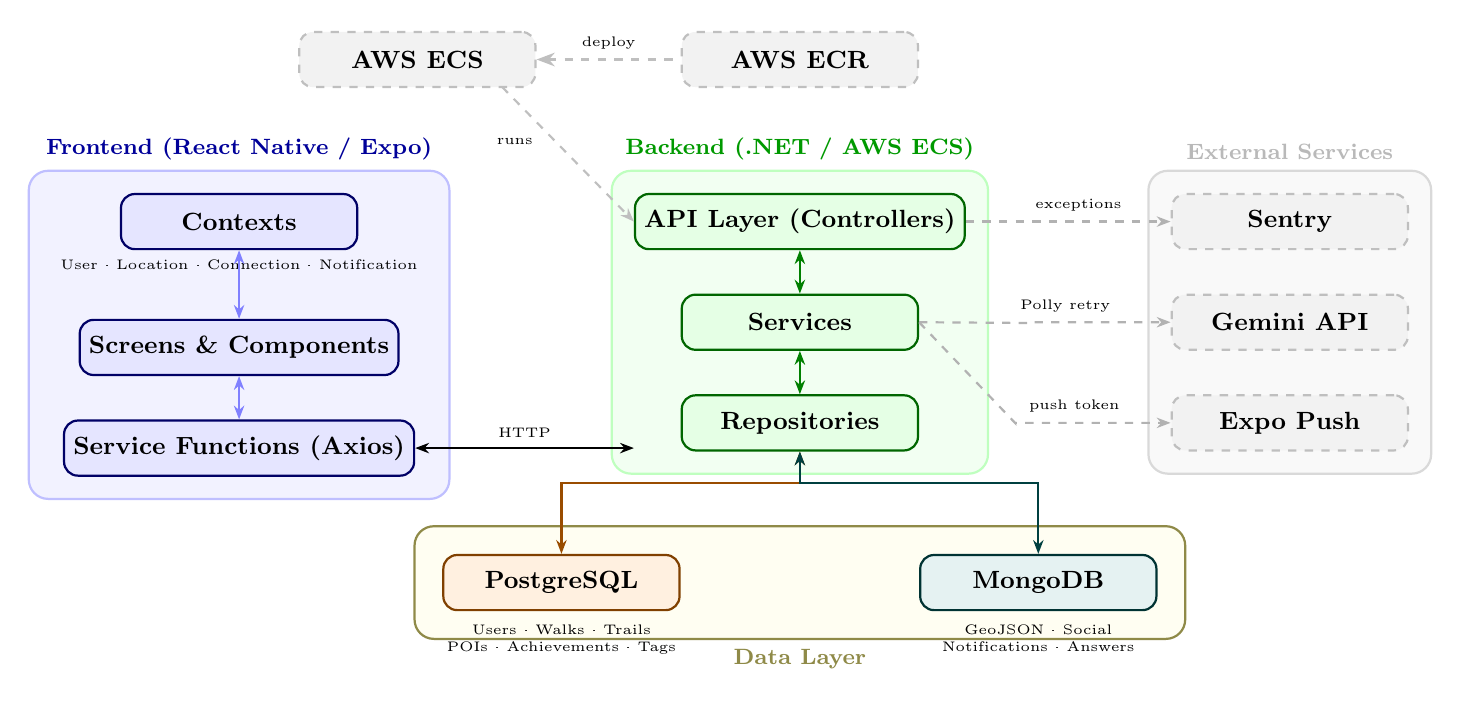
\begin{tikzpicture}[
    node distance=0.55cm and 1.4cm,
    box/.style={
        rectangle, rounded corners=5pt,
        minimum width=3.0cm, minimum height=0.7cm,
        text centered, font=\small\bfseries,
        draw=black!50, thick, fill=white
    },
    fe/.style={box, fill=blue!10, draw=blue!40!black},
    be/.style={box, fill=green!10, draw=green!40!black},
    db/.style={box, fill=orange!12, draw=orange!50!black},
    mg/.style={box, fill=teal!10, draw=teal!40!black},
    ex/.style={box, fill=gray!10, draw=gray!50, dashed},
    lbl/.style={font=\tiny, align=center},
    arr/.style={-{Stealth[length=5pt]}, thick},
    biarr/.style={{Stealth[length=5pt]}-{Stealth[length=5pt]}, thick},
]

%% ---- FRONTEND ----
\node[fe] (ctx)      {Contexts};
\node[lbl, below=0.0cm of ctx] (ctxlbl) {\tiny User · Location · Connection · Notification};
\node[fe, below=0.5cm of ctxlbl] (screens)  {Screens \& Components};
\node[fe, below=0.55cm of screens] (axiosvc) {Service Functions (Axios)};

%% ---- BACKEND ----
\node[be, right=3.5cm of ctx]           (ctrl) {API Layer (Controllers)};
\node[be, below=0.55cm of ctrl]         (svc)  {Services};
\node[be, below=0.55cm of svc]          (repo) {Repositories};

%% ---- DATABASES ----
\node[db, below left=1.3cm and 0.0cm of repo]  (pg)    {PostgreSQL};
\node[lbl, below=0.05cm of pg]  {\tiny Users · Walks · Trails\\ POIs · Achievements · Tags};

\node[mg, below right=1.3cm and 0.0cm of repo] (mongo) {MongoDB};
\node[lbl, below=0.05cm of mongo] {\tiny GeoJSON · Social\\ Notifications · Answers};

%% ---- EXTERNAL SERVICES ----
\node[ex, right=2.6cm of ctrl]           (gemini) {Sentry};
\node[ex, below=0.55cm of gemini]        (sentry) {Gemini API};
\node[ex, below=0.55cm of sentry]        (expo)   {Expo Push};

%% ---- AWS ----
\node[ex, above=1.33cm of ctrl]           (ecs)    {AWS ECR};
\node[ex, left=1.83cm of ecs]             (ecr)    {AWS ECS};

%% ---- FRONTEND INTERNAL ARROWS ----
\draw[biarr, blue!50] (ctx.south) -- (screens.north);
\draw[biarr, blue!50] (screens.south) -- (axiosvc.north);

%% ---- FE <-> BE ----
\draw[biarr, black, thick]
    (axiosvc.east) -- node[above, font=\tiny]{HTTP} (ctrl.west |- axiosvc.east);

%% ---- BACKEND LAYERS ----
\draw[biarr, green!50!black] (ctrl.south) -- (svc.north);
\draw[biarr, green!50!black] (svc.south)  -- (repo.north);

%% ---- REPO -> DBS ----
\draw[biarr, orange!60!black]
    (repo.south) -- ++(0,-0.4) -| (pg.north);
\draw[biarr, teal!50!black]
    (repo.south) -- ++(0,-0.4) -| (mongo.north);

%% ---- BACKEND -> EXTERNAL ----
\draw[arr, gray!60, dashed]
    (svc.east) -- ++(1.43,-0.01) |- node[font=\tiny, above left, pos=0.82, text=black]{Polly retry} (sentry.west);
\draw[arr, gray!60, dashed]
    (ctrl.east) -- node[font=\tiny, pos=0.55, above, text=black]{exceptions} (gemini.west);
\draw[arr, gray!60, dashed]
    (svc.east) -- ++(1.22,-1.28) |- node[font=\tiny, above, pos=0.69, text=black]{push token} (expo.west);

%% ---- CI/CD ----
\draw[arr, gray!50, dashed, arrows=Stealth-] (ecr.east) -- node[above, font=\tiny, text=black]{deploy} (ecs.west);
\draw[arr, gray!50, dashed] (3.34,1.71) -- node[font=\tiny, pos=0.31, below left, text=black]{runs} (ctrl.west);

%% ---- BACKGROUND ZONES ----
\begin{scope}[on background layer]
    \node[rectangle, rounded corners=7pt,
          fill=blue!5, draw=blue!25, thick, inner sep=8pt,
          fit=(ctx)(ctxlbl)(screens)(axiosvc),
          label={[font=\footnotesize\bfseries, blue!60!black]above:Frontend (React Native / Expo)}]
          (fezone) {};

    \node[rectangle, rounded corners=7pt,
          fill=green!5, draw=green!25, thick, inner sep=8pt,
          fit=(ctrl)(svc)(repo),
          label={[font=\footnotesize\bfseries, green!60!black]above:Backend (.NET / AWS ECS)}]
          (bezone) {};

    \node[rectangle, rounded corners=7pt,
          fill=yellow!5, draw=yellow!50!black, thick, inner sep=10pt,
          fit=(pg)(mongo),
          label={[font=\footnotesize\bfseries, yellow!50!black]below:Data Layer}]
          (dbzone) {};

    \node[rectangle, rounded corners=7pt,
          fill=gray!5, draw=gray!30, thick, inner sep=8pt,
          fit=(gemini)(sentry)(expo),
          label={[font=\footnotesize\bfseries, gray!55]above:External Services}]
          (exzone) {};
\end{scope}

\end{tikzpicture}
}
\caption{Application architecture: from the user's device to the databases and external services.}
\label{fig:architecture}
\end{figure}

\newpage
% ==========================================
% 3.3 Tasks Developed
% ==========================================
\subsection{Tasks Developed}
\label{sub:features}


% ==========================================
% Updating Project Resources
% ==========================================
\subsubsection{Updating Project Resources}
\label{subsub:updates}

One of the first things to tackle upon joining the project was to bring both repositories up to date.
Given how quickly these technologies are updated, several packages had fallen behind, and sorting them early was necessary before any real feature work could begin.
 
On the backend, the process was relatively straightforward.
The main change was upgrading the runtime to \textbf{.NET 10}, which introduced a new assertion API in the testing framework.
This meant going through the existing test suite and replacing the older \texttt{Assert.AreEqual(x,~y)} calls with the new \texttt{Assert.That(x,~Is.EqualTo(y))} style throughout.
The \textbf{MongoDB.Driver} package also required a version bump, but no code changes were required.
 
On the frontend, the problem was significantly more complex.
One of React Native's biggest strengths, its massive ecosystem of open-source packages, is also what makes dependency management so intricate: every package pulls in its own dependencies, and finding a combination of versions that are compatible is rarely simple.
To assist with this, the project used \textbf{Expo Doctor}, a tool built into the Expo CLI that scans all installed packages, flags version mismatches, and ranks conflicts according to severity.
 
What followed was a lot of digging through changelogs and documentation across multiple packages and both current and older versions, trying out different version combinations until things finally clicked.
One of the main culprits turned out to be a previously implemented offline-first feature that depended on a package named \texttt{watermelondb}, which had been fully deprecated and was simply no longer compatible with the current version of Expo.
In the end, the cleanest path forward was to comment out the entire feature, which got the app back into a working state, sacrificing offline and caching capabilities but opening up the path ahead.
 
This task was probably one of the hardest of the entire internship, not because it was conceptually difficult, but because it involved a lot of perseverance, reading across a wide range of documentation, and being able to find an equilibrium between the perfect fix and what was acceptable to scrap.

% ==========================================
% 3.3.2 Friends
% ==========================================
\subsubsection{Friend Lookup and Friend Requests}
\label{subsub:friends}

In Percursus, a social management framework allows users to search for peers via usernames and dispatch friend requests to them. I was tasked with optimizing the search functionality to look beyond strict, case-sensitive string literals and refactoring the user interface of the friend request system.

To address this limitation, a fuzzy matching, case-insensitive query approach was implemented.
Under this logic, search string inputs that are \textbf{only partially matching, misspelled, or variations of an existing username are dynamically resolved} rather than returning a null result if the username does not match perfectly.
This was achieved by restructuring the query that fetched a friend by exact username to use \texttt{ILIKE} in the username, first name, or last name field.

On the client side, the existing friend request system suffered from a fragmented user flow.
To resolve this issue, I designed a dedicated component to handle incoming friend notification payloads.
This provides clear and responsive interactive elements that allow users to seamlessly accept or reject pending requests with immediate visual feedback.
This refactoring unified the notification state machine with the user profile context, resulting in a significantly smoother and more intuitive interaction.

\begin{figure}[H]
    \centering
    \begin{minipage}[c]{0.48\textwidth}
        \centering
        
\includegraphics[width=\textwidth]{images/fuzzymatching.png}
        \caption{Fuzzy matching search component}
        \label{fig:friend_search}
    \end{minipage}
    \hfill
    \begin{minipage}[c]{0.48\textwidth}
        \centering
        
\includegraphics[width=\textwidth]{images/friends.png}
        \caption{Friend Request notifications}
        \label{fig:friend_request_ui}
    \end{minipage}
\end{figure}



% ==========================================
% 3.3.3 Leaderboard Improvements
% ==========================================
\subsubsection{Leaderboard Improvements}
\label{subsub:leaderboard}

For one of the gamification aspects of the application mentioned in Section~\ref{sub:sota:gamification}, after completing a trail, the user is placed on a leaderboard with its best completion time.
I was tasked with investigating and documenting how the leaderboard had previously been implemented, which turned out to be fairly lacking.

On the backend, there were methods missing from the \texttt{Service} and \texttt{Controller} layers with missing API endpoints.
The leaderboard itself was a list of every completed walk on a trail, sorted by a string representation of the duration of the walk, which is a mistake because sorting time intervals as strings with lexicographic ordering does not preserve the numeric order of the intervals.
The leaderboard had no concept of a best time per user, so every completed walk was returned and also had no concept of a user's friend, which made the results impersonal and suboptimal for readability.

To fix this, I rewrote the leaderboard query from scratch as a two-stage SQL query using Common Table Expressions (CTEs) that passed in a friends list, trail ID, and user ID.
The first stage uses \texttt{DISTINCT ON} to retain only each user's fastest time on a given trail, with the duration computed directly in the database as an interval rather than in application memory.
The second stage applies a \texttt{ROW\_NUMBER()} window function over the sorted results to assign each user a proper numeric rank.
The final result is then filtered to return only the top five finishers, plus the current user's entry and any friends' entries regardless of rank, so the leaderboard always feels relevant to whoever is looking at it.

On the frontend, the feature was much more complete, only needing to update the strings in time to seconds, current user and friends badges to distinguish them, and a new UI look to display a podium of the top three and adding the leaderboard of each trail to its own detail \texttt{View}.
 
The end result was a leaderboard that returned correct, meaningful data: best times only, properly ranked, and filtered to the handful of entries that actually matter to the user.

\begin{figure}[H]
    \centering
    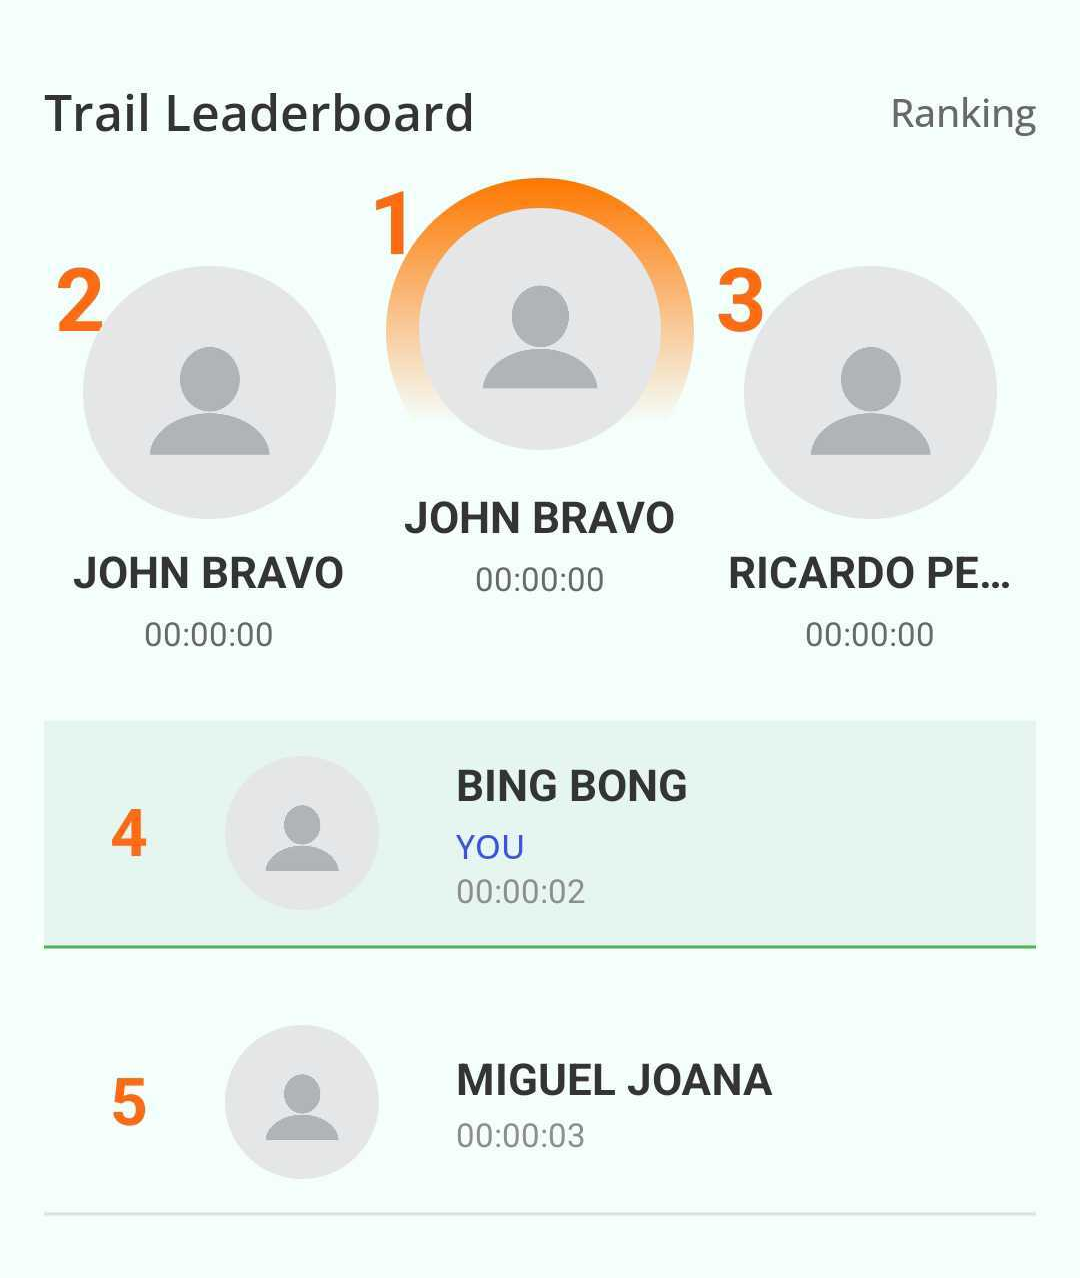
\includegraphics[width=0.5\textwidth]{images/leaderboard.png}
    \caption{Trail Leaderboard Instance}
    \label{fig:leaderboard}
\end{figure}


% ==========================================
% 3.3.4 User Settings and Account Settings
% ==========================================
\subsubsection{User and Account Settings}
\label{subsub:settings}

Like any other application with users, each must have their credentials and personal information editable and correctly stored.
A user's profile in Percursus includes a profile picture, display name, email address, date of birth, question difficulty preference, and a summary of their activity: number of trails completed, achievements earned, and friends added.
 
However, this was not the case when I first started.
Several of these fields were either hardcoded on the frontend, did not properly flow through the full backend stack, or simply missed the plumbing to connect the UI to the database.
 
On the backend, most of the endpoints already existed; therefore, the work was less about building from scratch and more about ensuring that the data were correctly crossing every layer, from the request body, through the service and repository layers, and into the database.
The main additions were a new endpoint for updating the user's question difficulty preference, which was missing entirely, and a new endpoint for creating achievements.
Everything else required tracing the existing flow, identifying where values were being dropped or ignored along the way, and fixing the gaps.

\begin{figure}[H]
    \centering
    \begin{minipage}[c]{0.48\textwidth}
        \centering
        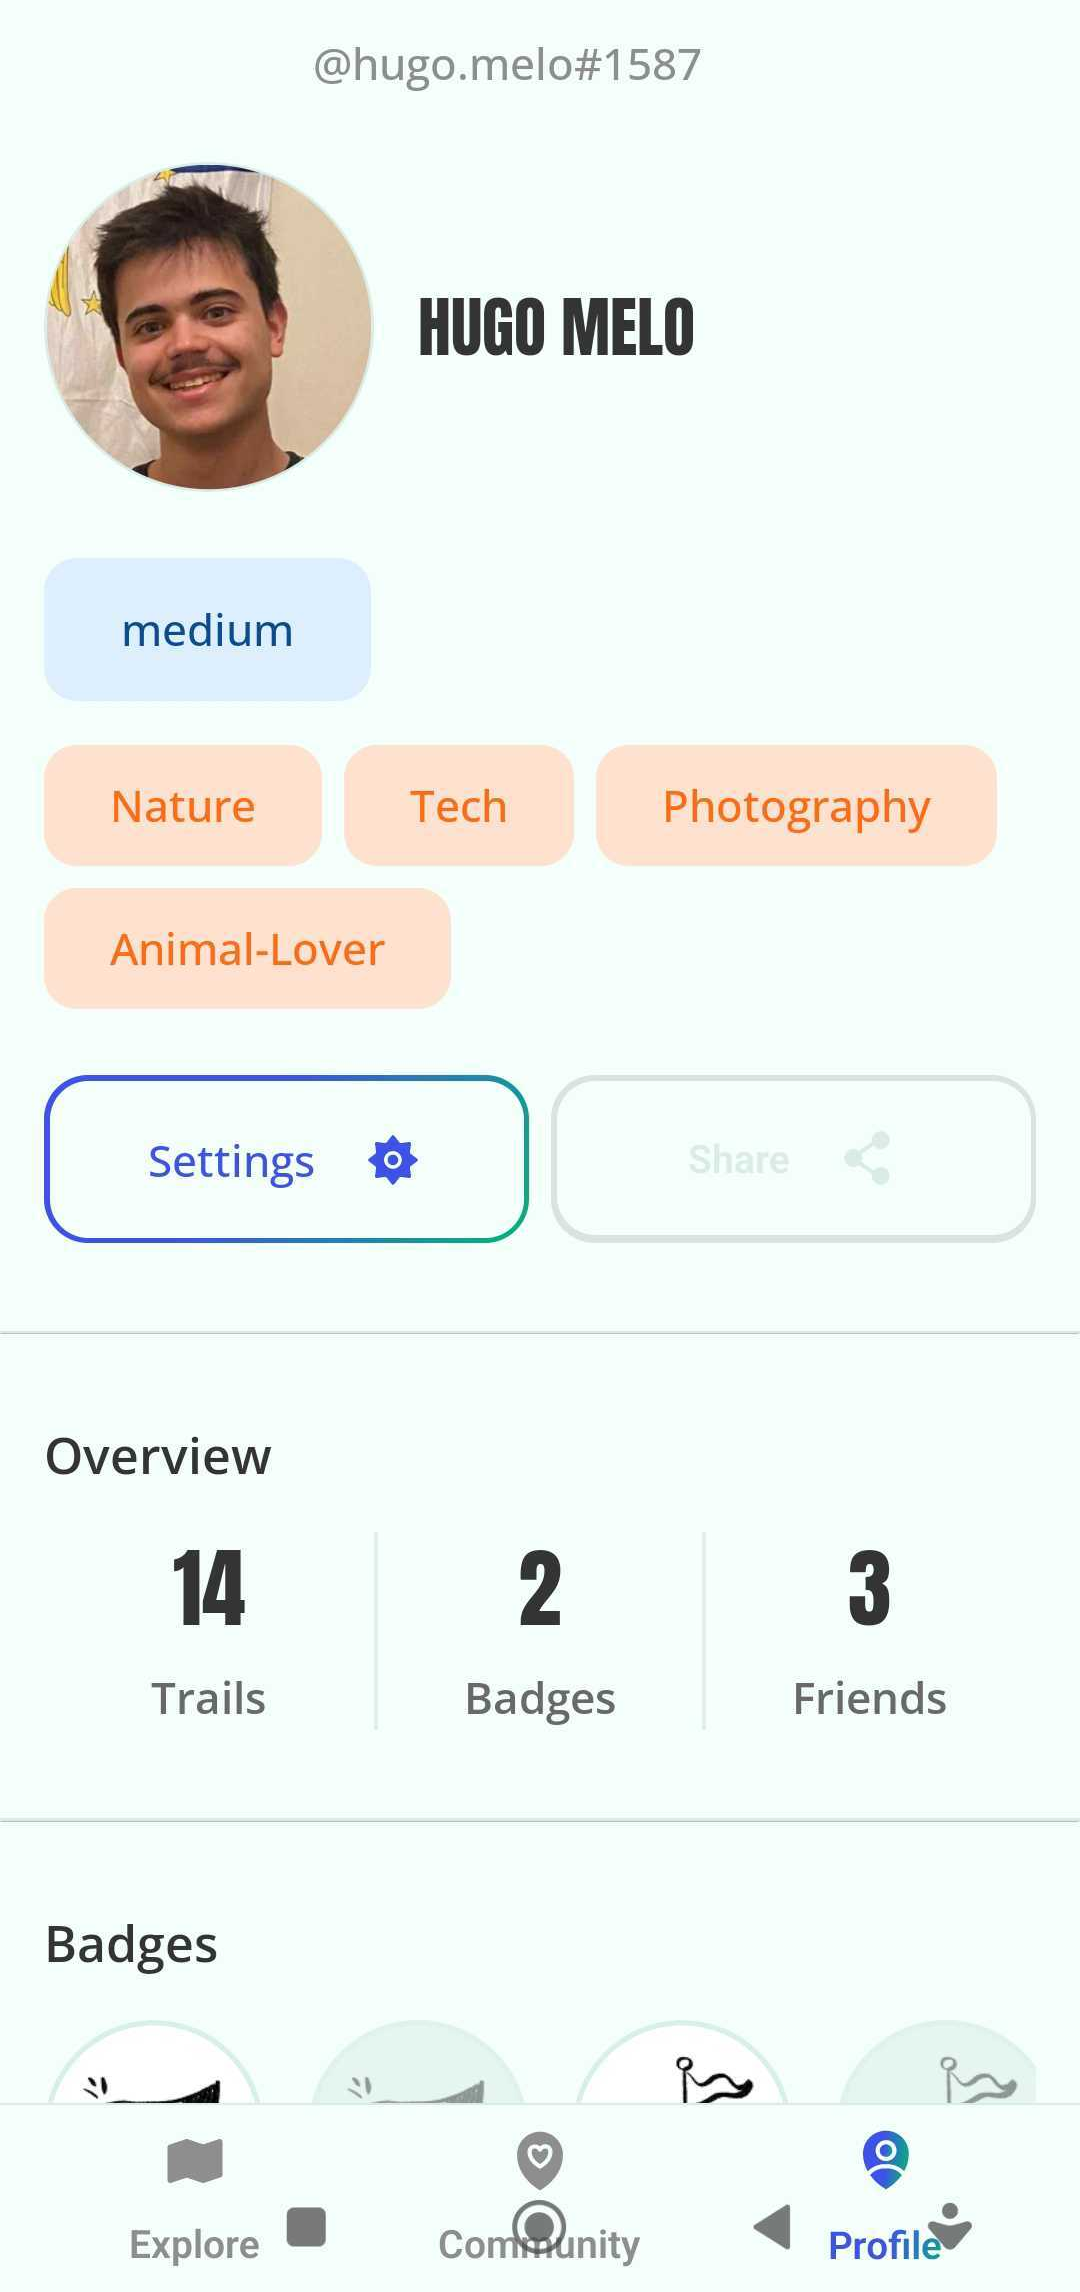
\includegraphics[width=\textwidth]{images/accountview.png}
        \caption{User's Profile View interface.}
        \label{fig:accountview}
    \end{minipage}
    \hfill 
    \begin{minipage}[c]{0.48\textwidth}
        \centering
        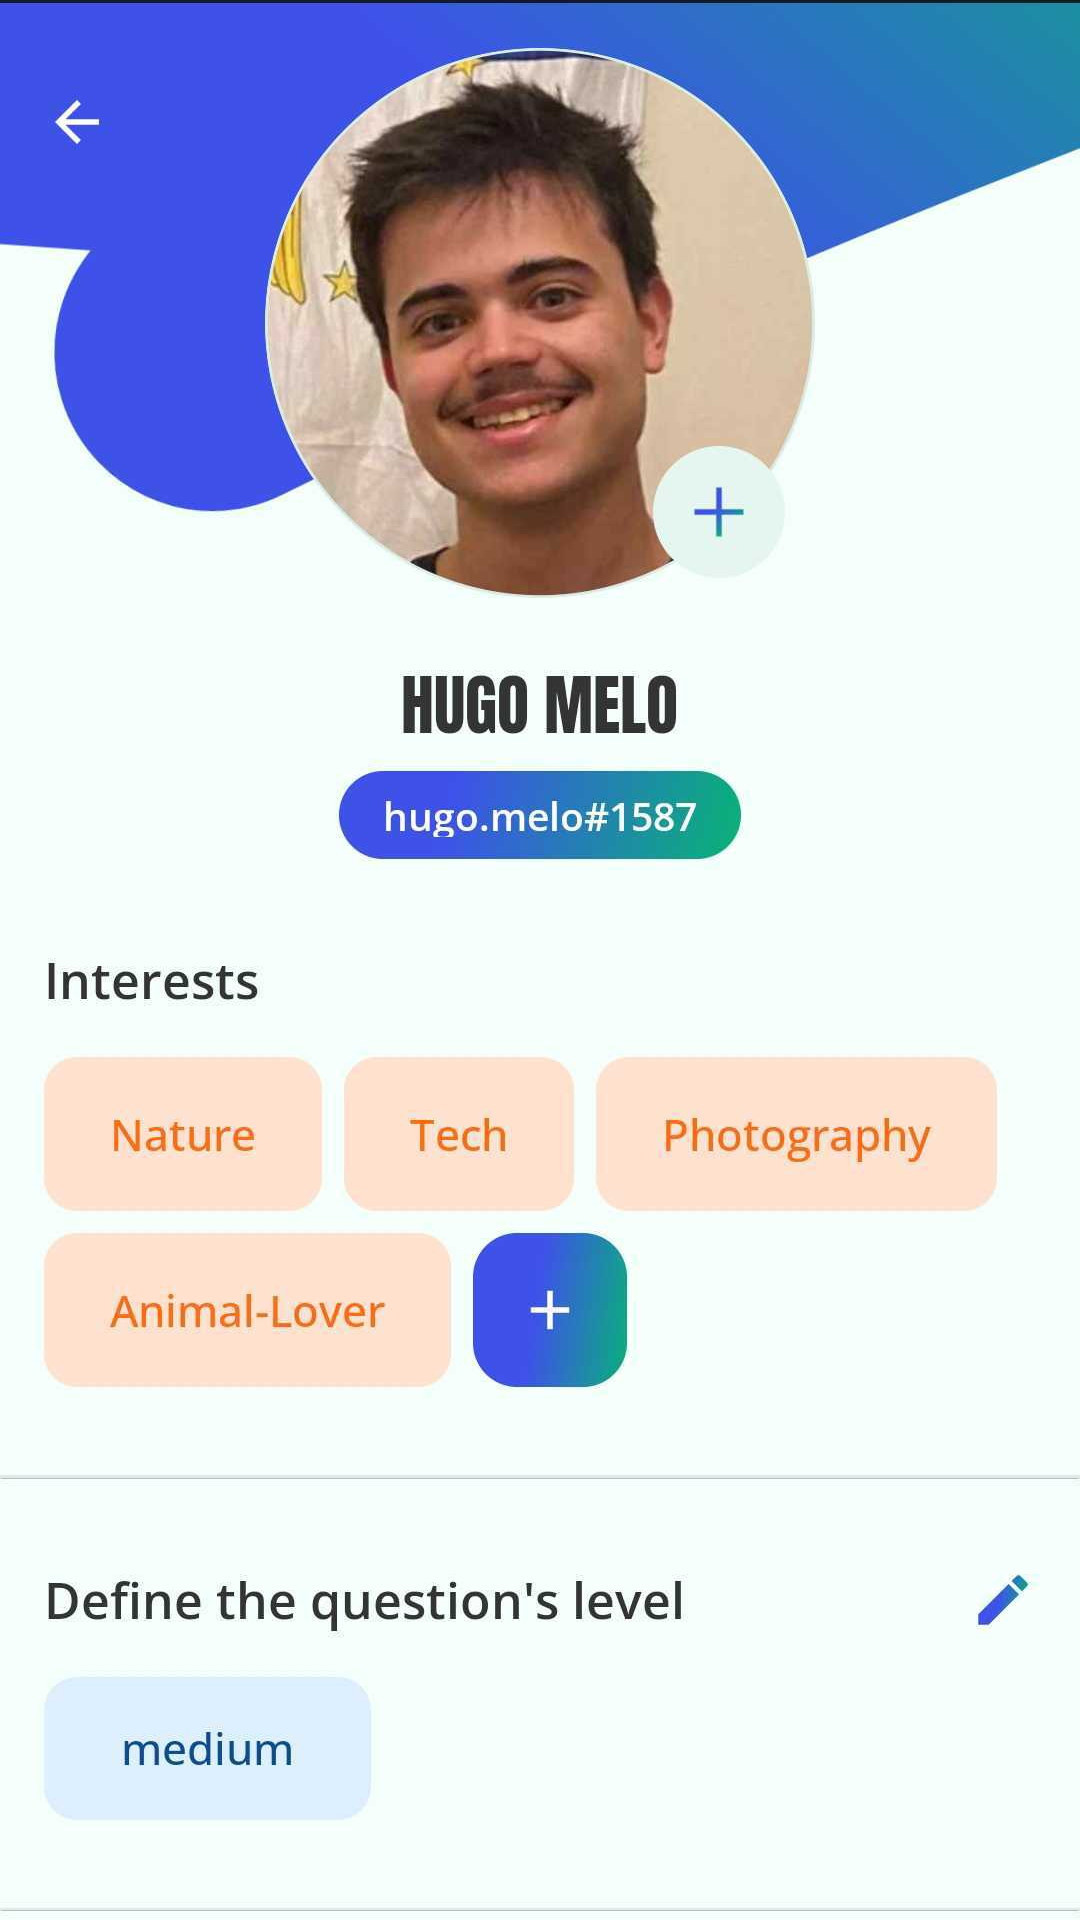
\includegraphics[width=\textwidth]{images/settingsview.png}
        \caption{Application settings and user preferences.}
        \label{fig:settingsview}
    \end{minipage}
\end{figure}
 
On the frontend, the profile overview screen had several fields displaying hardcoded placeholder values rather than real data: date of birth, number of completed trails, number of achievements, and number of friends.
These were wired up to the appropriate API calls, so they now reflect the actual state of the user's account.
 
The profile photo upload required more attention.
The original implementation sent the image as a full base64 string prefixed with the data URI scheme (\texttt{data:image/jpeg;base64,...}), which was stored as-is in the database.
The fix involved separating the raw base64 payload from the prefix before sending it and adding a size check on the client side: if the encoded image exceeded a set maximum length, the upload was rejected early with a \texttt{Toast} notification rather than letting an oversized payload reach the API. Profile photos are stored as raw base64 directly in the database, which is functional for the current stage of the project but is not ideal at a larger scale.
The natural next step would be to migrate photo storage to an object storage service such as AWS S3, keeping only the URL in the database rather than the binary content itself.

\begin{figure}[H]
    \centering
    \begin{minipage}[c]{0.48\textwidth}
        \centering
        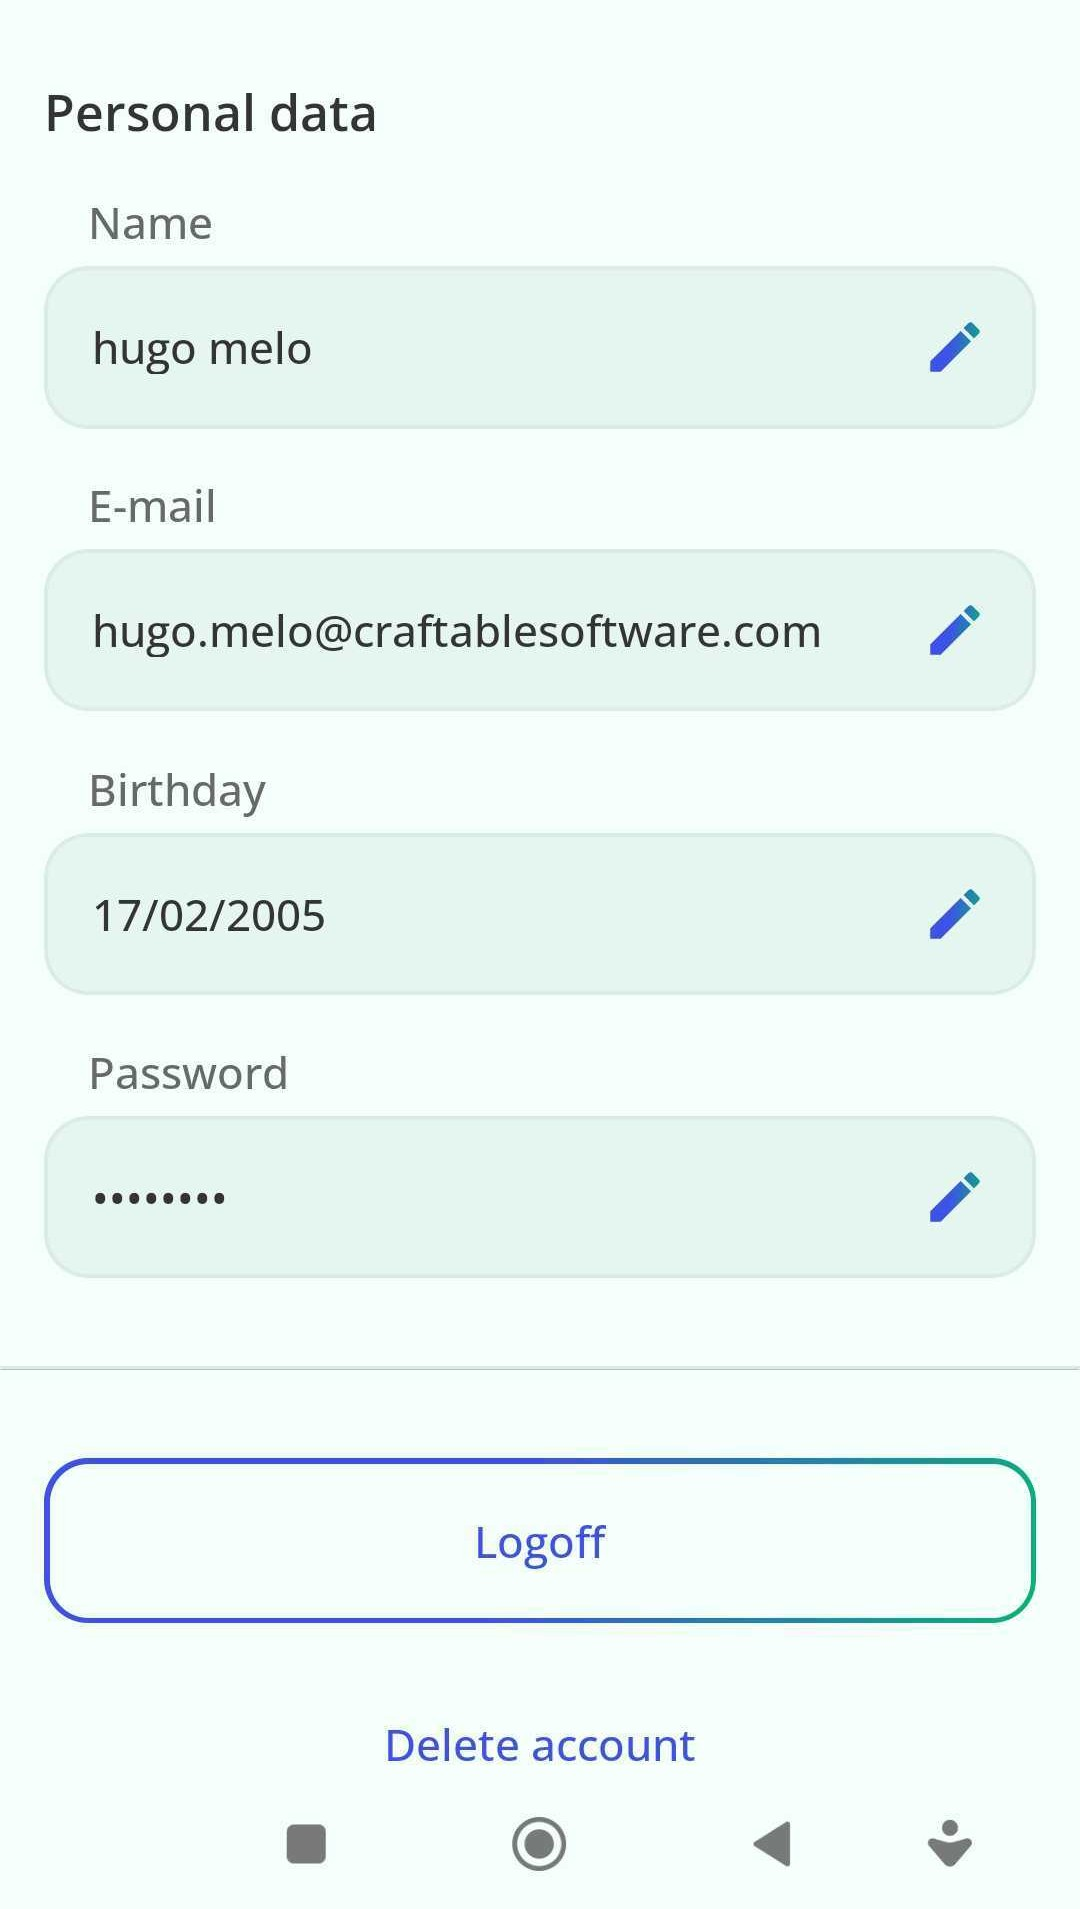
\includegraphics[width=\textwidth]{images/personaldata.png}
        \caption{Personal data management configurations.}
        \label{fig:personaldata}
    \end{minipage}
    \hfill 
    \begin{minipage}[c]{0.48\textwidth}
        \centering
        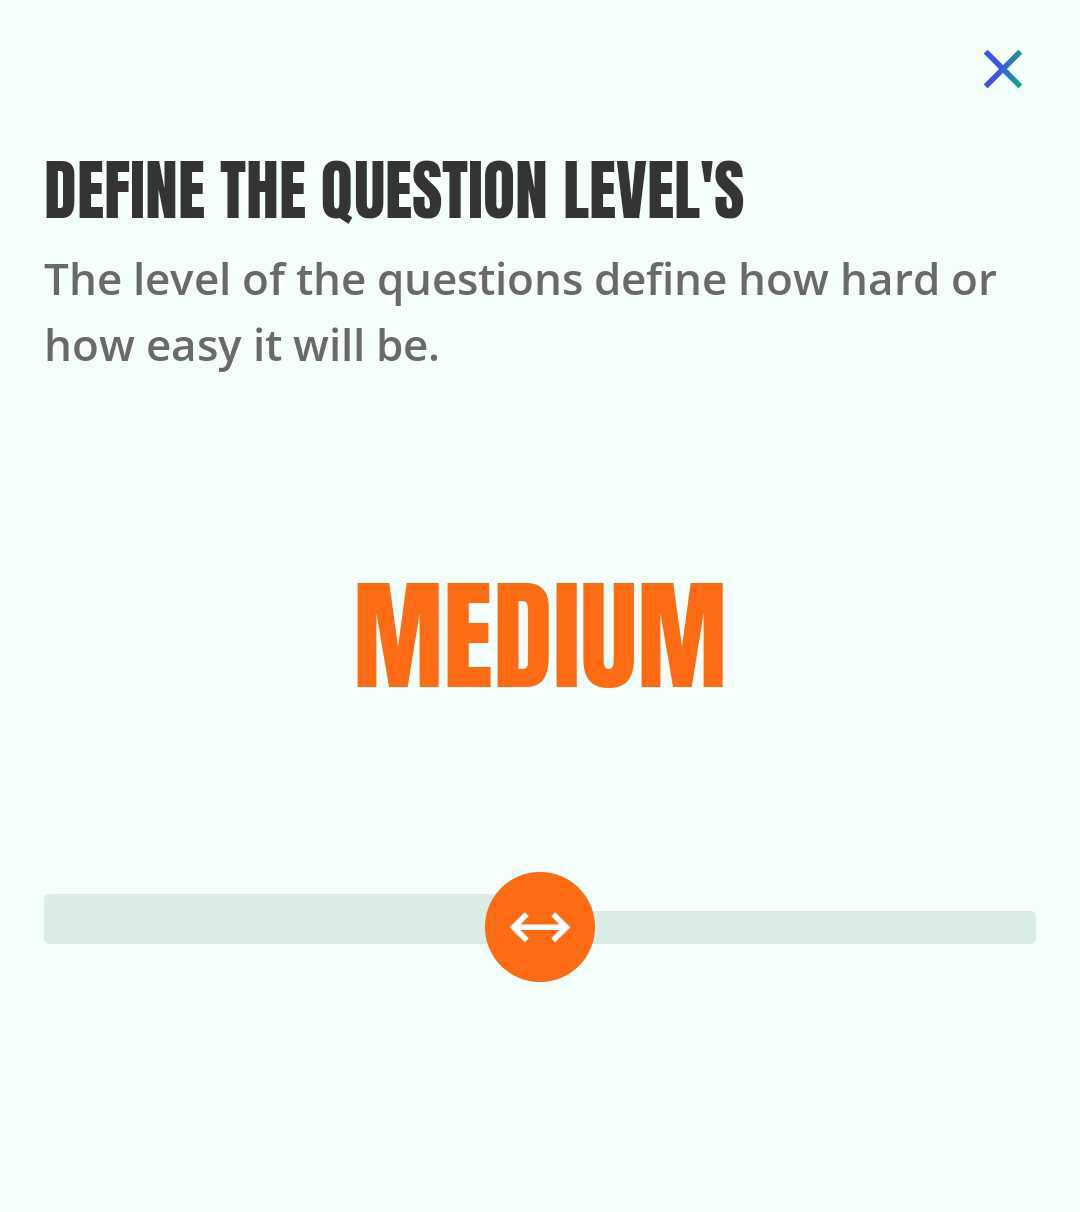
\includegraphics[width=\textwidth]{images/questionlevel.png}
        \caption{Question tier selection and categorization UI.}
        \label{fig:questionlevel}
    \end{minipage}
\end{figure}


% ==========================================
% AI Questions Integration
% ==========================================
\subsubsection{AI Quiz Feature}
\label{subsub:ai}

This feature replaced a static quiz model (one hardcoded question set per Point of Interest) with dynamic generation, so that each trail could scale without manually authoring large question banks.
The final implementation was not built in one pass; it evolved through several iterations, and most of the work was focused on improving geospatial accuracy and response latency.

\paragraph{Model Selection}
Before implementation, I compared Google Gemini 3.1 Pro, OpenAI GPT-5.4, Anthropic Claude 4.6 Sonnet, and DeepSeek V4 in terms of reasoning quality, geospatial grounding, context window, cost, and C\# integration.
The deciding requirement was \textbf{location fidelity}: for a trail app, a question about the wrong monument is a critical product error.

Gemini 3.1 Pro was selected because it was the only evaluated model with native Google Maps grounding support, which is better aligned with POI-level validation than generic web search grounding.
It also had competitive economics (\$2.00/\$12.00 per million input/output tokens), a large context window, and fit cleanly into the backend through \texttt{Google.Cloud.VertexAI.Extensions} and \texttt{Microsoft.Extensions.AI}, keeping the service layer provider agnostic.

\paragraph{Implementation Iterations}
This was my first and most significant feature in the project, so I developed it incrementally:

\begin{enumerate}
    \item \textbf{Mocked backend flow first.} I implemented service methods and contracts with mocked responses (no database fetch yet) to quickly validate the endpoint design, response DTO shape, and error handling.

    \item \textbf{Database integration.} After the contract was stabilized, I replaced the mocks with real data retrieval (trail/POI/user context), which became the payload foundation for prompt construction.

    \item \textbf{Frontend integration.} Once the API path was stable, the frontend flow for question display and answer submission was wired.

    \item \textbf{Accuracy debugging and prompt hardening.} Initial end-to-end tests revealed a major issue: when the user was near a POI, the generated question was often about a nearby landmark, not the intended point.

    \item \textbf{Latency optimization via preloading.} Even after improving accuracy, on-demand generation still introduced a visible delay when users approached POIs.
\end{enumerate}

\paragraph{Accuracy Issue and Resolution}
The key failure mode was ambiguity in the geospatial context.
Early prompts used user-nearby coordinates with lower precision, which gave the model too much room to choose semantically related but incorrect landmarks.

I addressed this with stricter prompt constraints and more precise coordinate semantics:

\begin{itemize}
    \item increased coordinate formatting from 6--8 variable decimals to fixed \textbf{7 decimal places} and explicitly declared \textbf{WGS84};
    \item added a hard proximity rule (the referenced POI must be within \textbf{10 meters});
    \item strengthened instruction language to reduce model freedom (critical-task framing);
    \item introduced a \textbf{priority list} (exact building first, then exact monument/statue, then unique architectural feature, and only then surrounding area).
\end{itemize}

The resulting behavior was significantly more consistent with the intended POI, reducing incorrect landmark questions during field testing.

\paragraph{Latency Issue and Architectural Change}
After accuracy improvements, the next bottleneck was the user-perceived delay.
Originally, the app generated each question only when the user entered the POI radius.
This on-demand call path made the latency visible in the UI.

To solve this, I changed the flow from \textit{reactive generation} to \textit{asynchronous preloading}:

\begin{itemize}
    \item when a user starts a trail, the backend asynchronously generates questions for all trail POIs in advance;
    \item generation now uses \textbf{POI coordinates} directly (instead of transient user coordinates), which also improved accuracy;
    \item generated items are cached for the active trail session and discarded if the user exits the trail;
    \item at interaction time, the app reads preloaded questions, so the remaining real-time latency is mainly the answer-validation call.
\end{itemize}

Because LLM calls are asynchronous, the API returns HTTP \texttt{202 Accepted} while generation jobs are running, and the frontend transitions to loading/polling states rather than blocking them.
Rate limiting and retry policies were implemented with \textbf{Polly} exponential backoff, consistent with other outbound HTTP integrations in the backend.

\paragraph{Prompt Evolution}
To make the iteration process explicit, the prompt was developed through three practical versions:

\begin{itemize}
    \item \textbf{V1 (baseline):} generic request to create a quiz question from user location and profile context. This version functioned well but frequently selected nearby, non-target landmarks.
    \item \textbf{V2 (accuracy-focused):} introduced fixed coordinate precision (7 decimals), explicit WGS84 reference, and stronger imperative wording around exact-coordinate interpretation.
    \item \textbf{V3 (production):} added a hard 10-meter validity rule, explicit title constraint (must contain the exact place name), and a priority hierarchy for POI identification.\\
\end{itemize}

The two images below are the first and last iteration of the context prompt:\\

\begin{figure}[H]
    \centering
    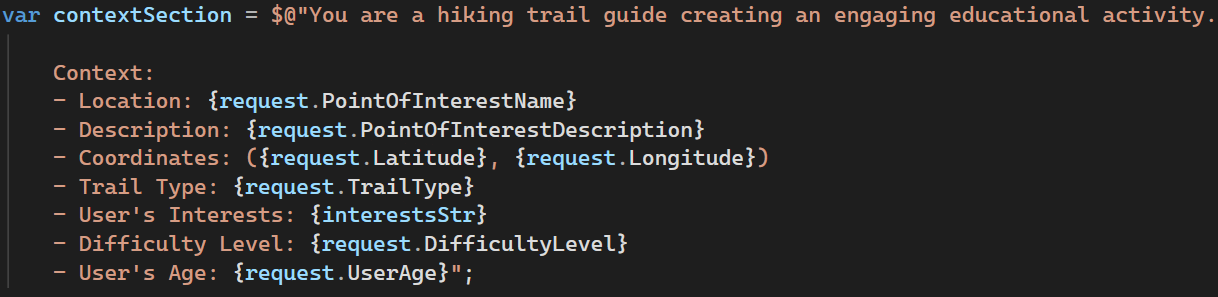
\includegraphics[width=1\textwidth]{images/prompt1.png}
    \caption{Context Prompt: First Iteration}
    \label{fig:prompt1}
\end{figure}

\begin{figure}[H]
    \centering
    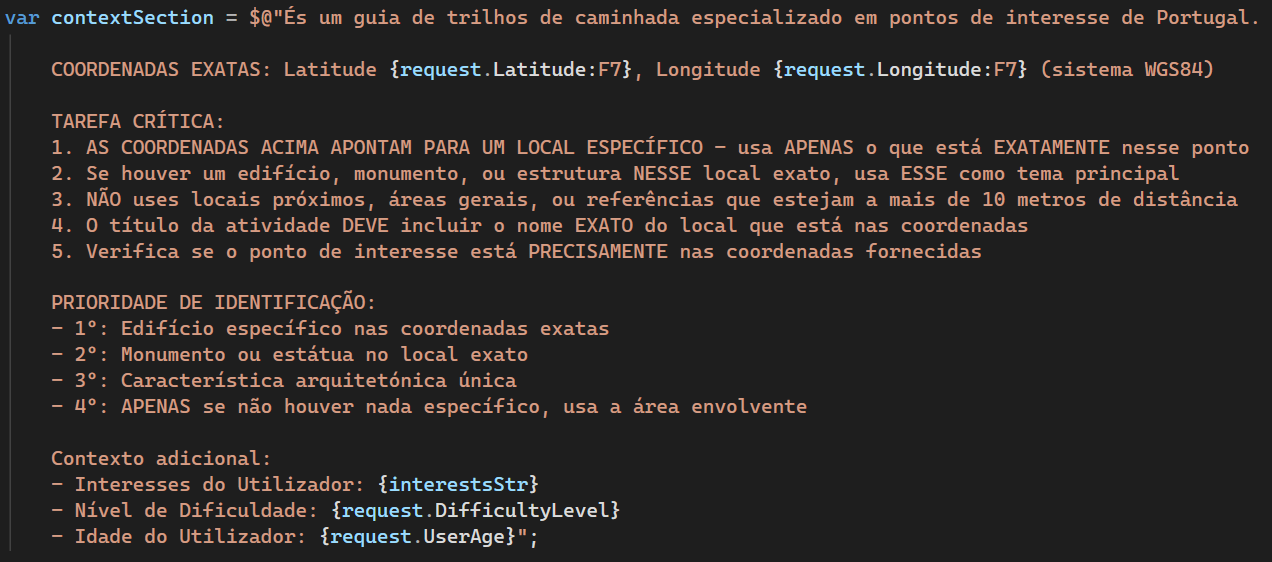
\includegraphics[width=1\textwidth]{images/prompt2.png}
    \caption{Context Prompt: Last Iteration}
    \label{fig:prompt2}
\end{figure}

\paragraph{Answer Validation}
 
Displaying the question was only part of this feature.
The other was validating the user's answer, which introduced an interesting challenge: for multiple-choice questions, a simple equality check suffices, but for open-ended questions, there is no single correct string to compare against.
Rather than hardcoding the validation logic, answer validation was delegated to the LLM via a second prompt.
The backend sends the original question, the expected answer context, and the user response and asks the model to assess whether the answer is correct.
This keeps validation flexible and consistent with the generative nature of the questions, at the cost of a second API call per answer submission.

\begin{figure}[H]
    \centering
    \begin{minipage}[c]{0.48\textwidth}
        \centering
        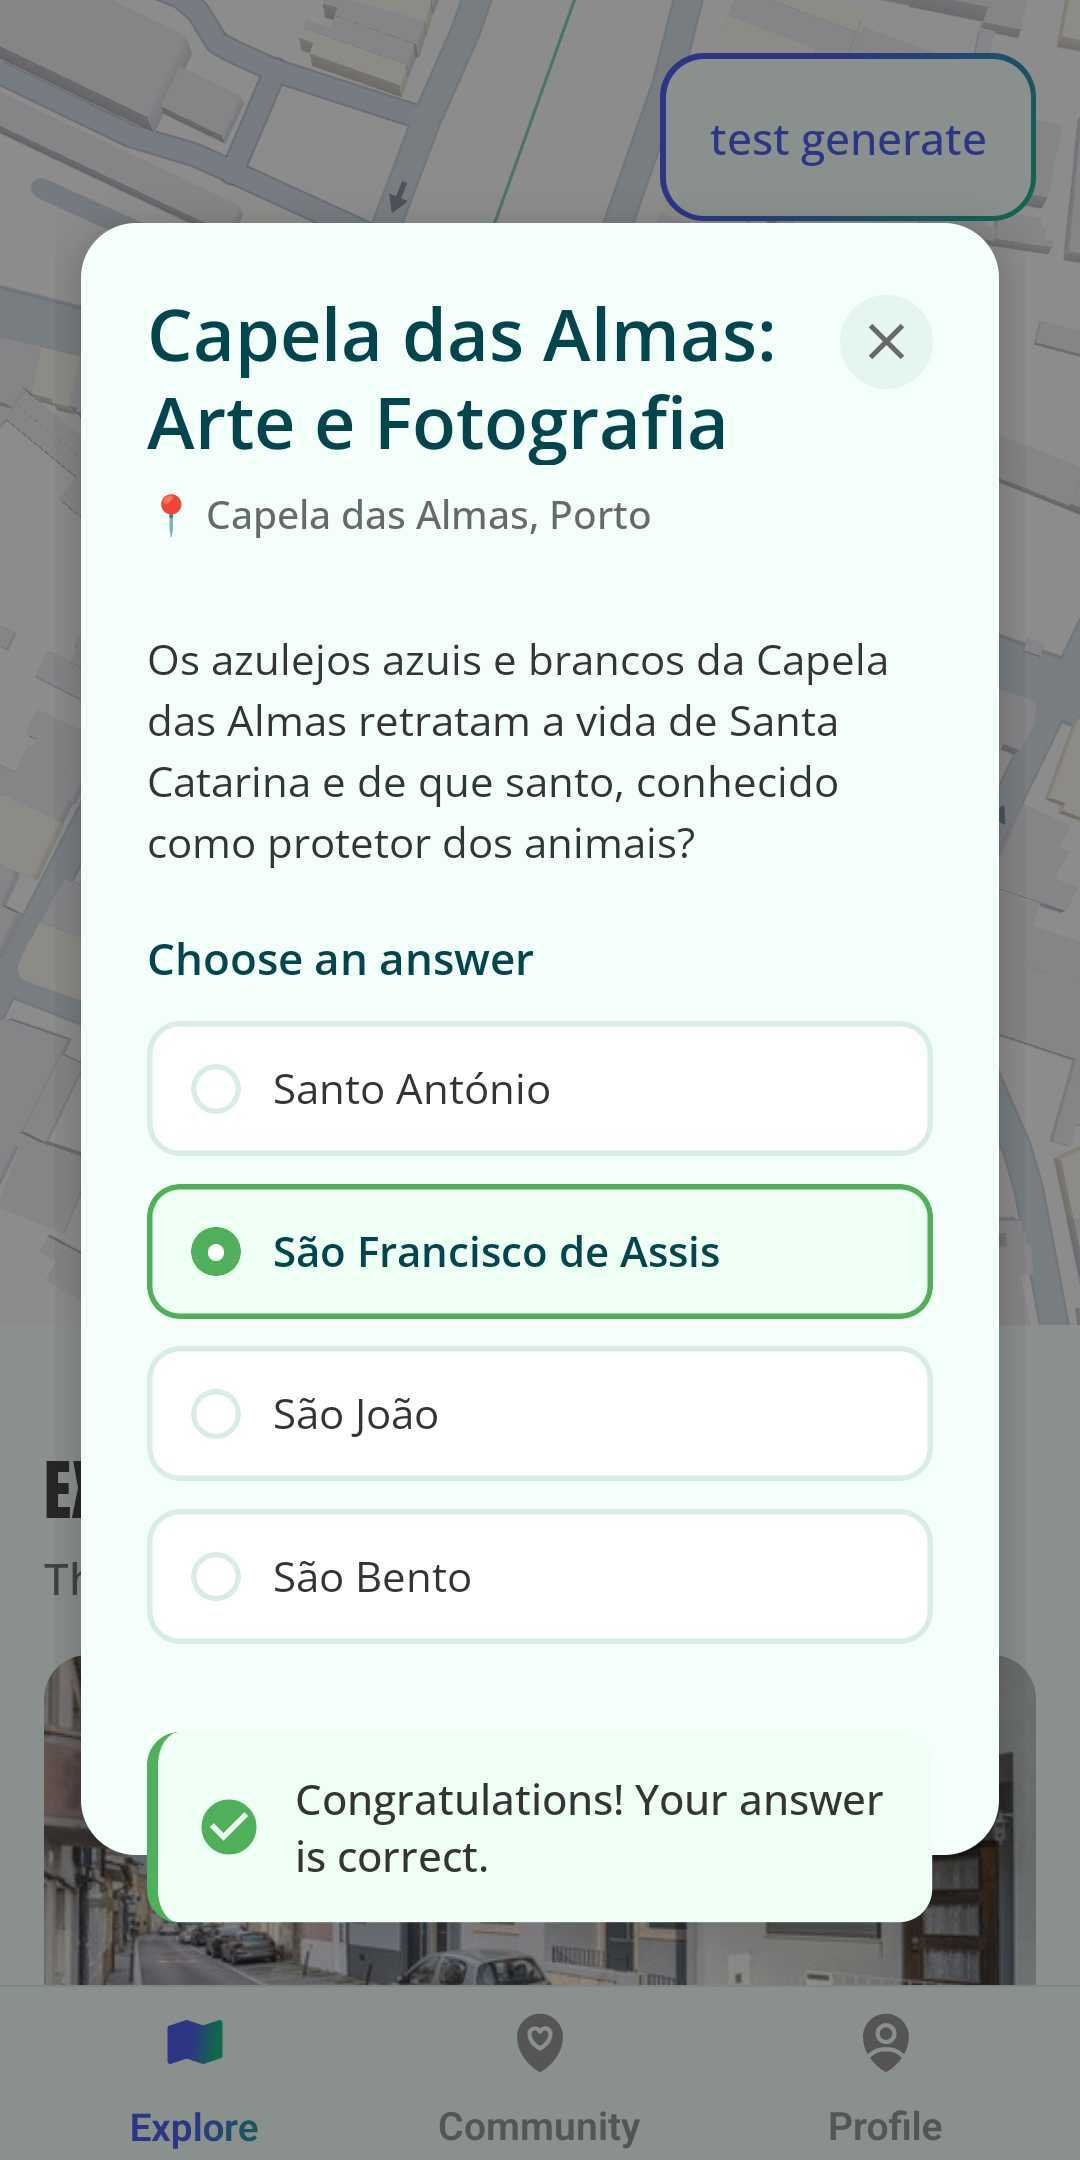
\includegraphics[width=\textwidth]{images/ai_correct.png}
        \caption{Correct Multiple Choice Question}
        \label{fig:ai_correct}
    \end{minipage}
    \hfill 
    \begin{minipage}[c]{0.48\textwidth}
        \centering
        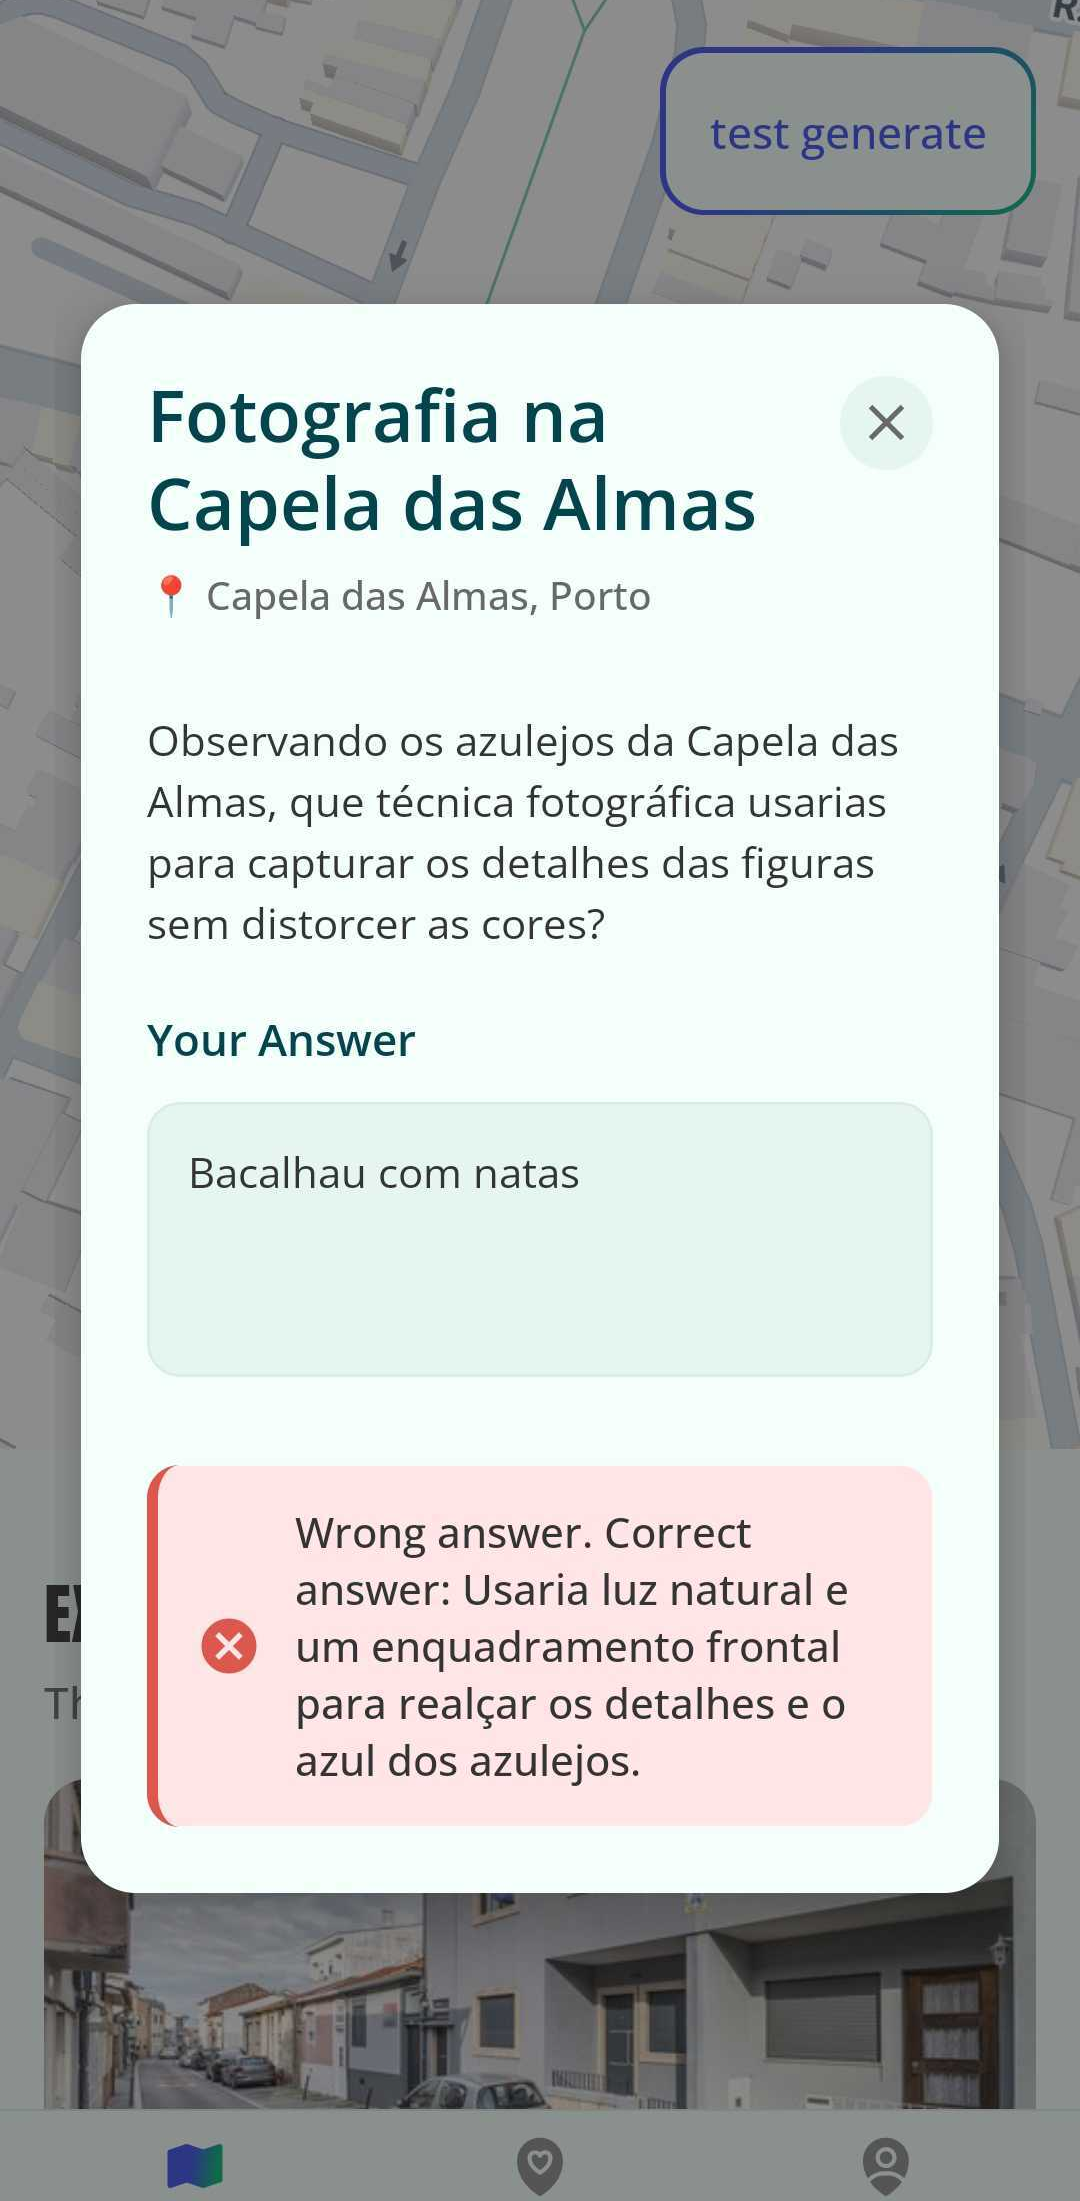
\includegraphics[width=\textwidth]{images/ai_wrong.png}
        \caption{Incorrect Open Ended Question}
        \label{fig:ai_wrong}
    \end{minipage}
\end{figure}

\newpage

% ==========================================
% Future Work
% ==========================================
\section{Future Work}
\label{sec:future}
 
While the internship covered significant ground across the application's core features, several items remain on the roadmap for future development iterations. \\

\textbf{AI quiz resilience and next iteration scope.}
 The feature currently covers the full operational loop: context ingestion, asynchronous preloading, question serving, answer validation, and failure handling.
The two main risks identified during implementation were (1) location accuracy and (2) runtime latency, both of which were reduced through prompt hardening and the preload solution.

First, native geospatial grounding and multimodal challenges (for example, photo-based identification of signs or ecological features) have not yet been activated.
Second, despite preloading improvements, the feature still depends on connectivity for generation and validation.
A practical production strategy is a \textbf{hybrid fallback}: the online mode uses Gemini-generated content, and the offline/degraded mode serves a curated local question set from the database.
This preserves playability on low-signal trails, reduces token spending, and maintains static content as a resilience layer instead of deprecating it.\\
 
\textbf{Point system and unified leaderboard.}
The current leaderboard ranks users by their trail completion time.
The intended design is a broader point system in which users accumulate points across multiple dimensions: trail completions, correct quiz answers, achievements earned, and streaks.
The leaderboard should then reflect this cumulative score rather than time alone, making it more engaging and harder to complete by simply rushing through a trail.\\
 
\textbf{Dynamic achievement creation.}
A proof of concept for dynamically generating and assigning achievements based on user behaviour is planned.
The current implementation has a fixed set of achievement types defined
at the database level.
The goal is to make achievement creation data-driven, either through a configuration layer or an LLM-assisted generation flow similar to the one already in place for quiz questions.\\
 
\textbf{CMS development.}
A content management system for trail and POI administration is partially implemented and needs to be continued.
Trail managers and administrators should be able to add, edit, and publish trails, points of interest, and associated metadata without directly touching the database.
This is a prerequisite for the platform to be scaled beyond the development team.\\
 
\textbf{Google authentication.}
Google sign-in is partially scaffolded in the backend but is not functional in the current build version. The root issue is that the Expo Go client does not support custom native modules required for a proper OAuth flow.
Moving to a development build (a custom compiled version of the app that is not constrained by Expo Go's sandbox) would unblock this, and it is the recommended next step for authentication in general, given that the application currently has no token-based authentication layer at all.\\
 
\textbf{Offline-first implementation.}
As mentioned in earlier sections, the offline-first capability was broken by upstream React Native and Expo updates and moved to the backlog. 
Restoring it is a priority for any production release, given that trails are, by definition, used in environments where connectivity is unreliable.
The fix will require migrating away from the deprecated package to a supported alternative and should be paired with the LLM hybrid fallback strategy discussed in Section~\ref{subsub:ai}: serving cached questions from the database when the device is offline rather than failing the quiz entirely.\\
\newpage
 
\textbf{Frontend CI pipeline and automated testing.}
The frontend repository currently has no automated testing suite or CI pipeline. Adding one is the most straightforward gap to close relative to the state-of-the-art and would have prevented the offline-first regression from going undetected.
Introducing even a basic suite of component and integration tests, gated on pull requests via Bitbucket Pipelines, would bring the frontend in line with the backend delivery maturity.\\
 
\textbf{Profile photo migration to cloud storage.}
Profile photos are currently stored as raw base64 strings in PostgreSQL, which is functional but does not scale well.
Migrating to an object storage service, such as AWS S3, with only the URL persisted in the database, is a natural and relatively contained improvement that would reduce the database size and improve the image load performance.

\vspace*{1cm}

% ==========================================
% CONCLUSION
% ==========================================
\section{Conclusion}
\label{sec:conclusion}
 
The application developed throughout this internship sits at an interesting intersection of the trends surveyed in Section~\ref{sec:sota}: it combines location-based outdoor exploration, gamified engagement mechanics, AI-generated content, and a social layer built around friends and leaderboards, all areas where the industry is actively investing and user expectations are rising fast.
Looking back at the established benchmarks, the project holds up well.
The core gamification loop, which ties leaderboards and achievements to real POI activities rather than arbitrary actions, reflects the hybrid reward architecture that the literature identifies as the most effective for retention.
LLM integration addresses the content scalability problem that any location-based trivia system inevitably faces, and the choice of Gemini 3.1 Pro positions the feature to grow into richer geospatial grounding and multimodal challenges as the platform matures.
The gaps that remain, most notably offline-first regression and the absence of frontend automated testing, are real but well understood, and both have a clear path forward.\\
 
On a personal level, this internship was one of the most formative experiences I have ever had.
Coming in, I had a reasonable theoretical foundation but limited exposure to what a real, production-bound codebase actually looked like: the architectural decisions, the trade-offs, and the unglamorous-but-necessary work of fixing dependency trees or tracing a value that gets dropped somewhere between a service and a repository.
Working across two repositories, in two different languages and ecosystems, on features that ranged from database query design to LLM prompt engineering, gave me practical experience that is hard to replicate outside of a real project.
More than any specific technology, I gained a better intuition for how good software is structured, developed with clear documentation for the next developer, and with the user's interest in mind.

\newpage

% ==========================================
% BIBLIOGRAPHY
% ==========================================
\bibliographystyle{alpha}
\bibliography{references}

\end{document}



